\subsection{E4 -- Anomaly scenarios}
\begin{figure*}[t]
\centering
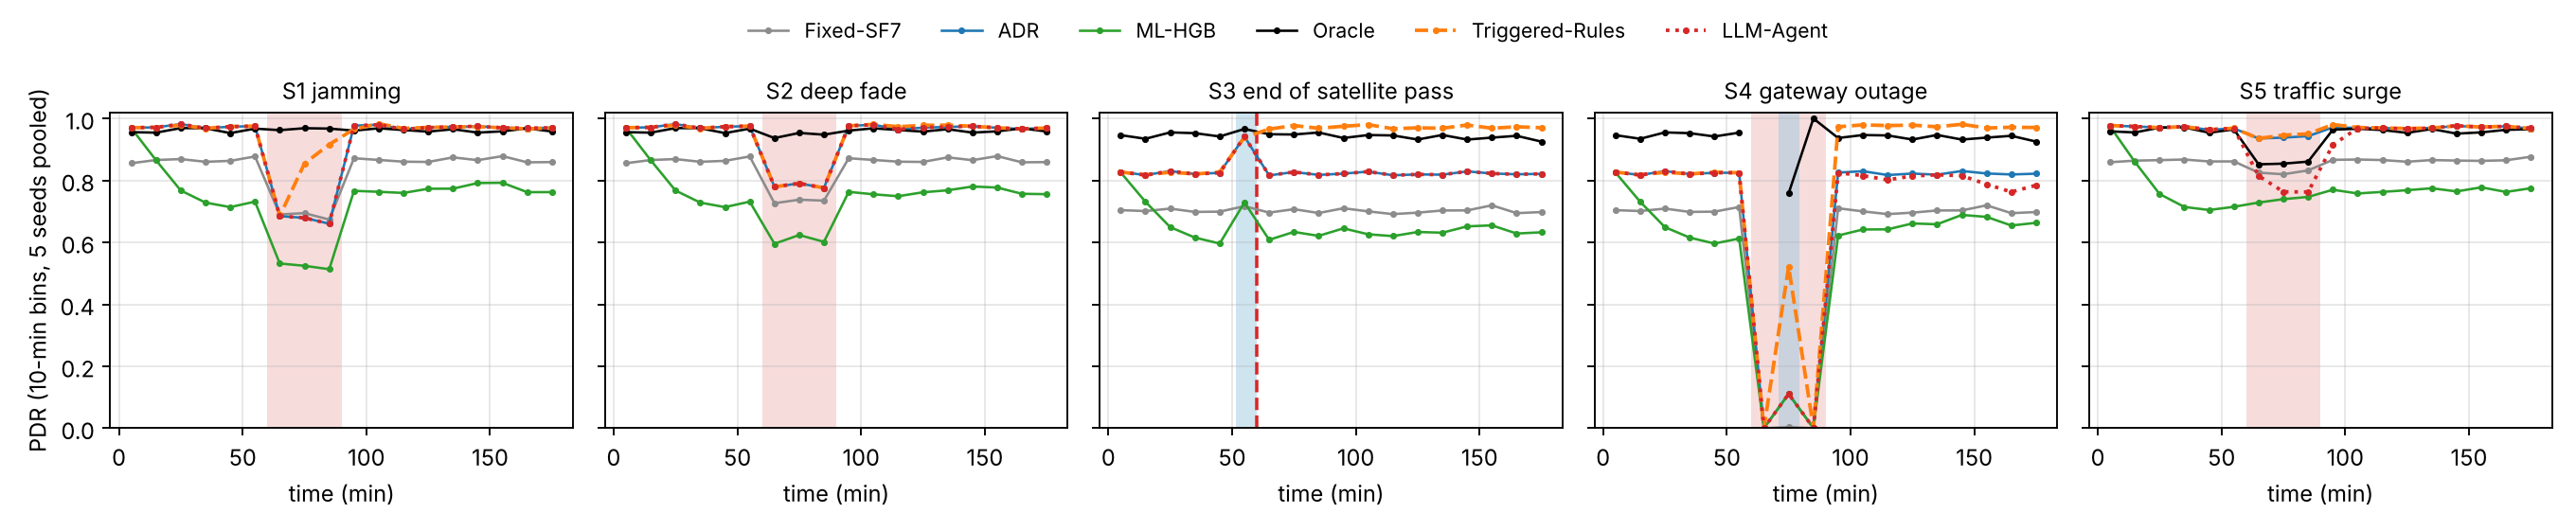
\includegraphics[width=\textwidth]{../results/e4_pdr_timeline_wide.png}
\caption{E4. PDR over time around the five events (10-min bins pooled over 5 seeds; red: event,
blue: satellite pass). Fixed SF12 is off-scale and omitted. LLM agent: Qwen3-0.6B.}
\label{fig:e4}
\end{figure*}
\begin{figure}[t]
\centering
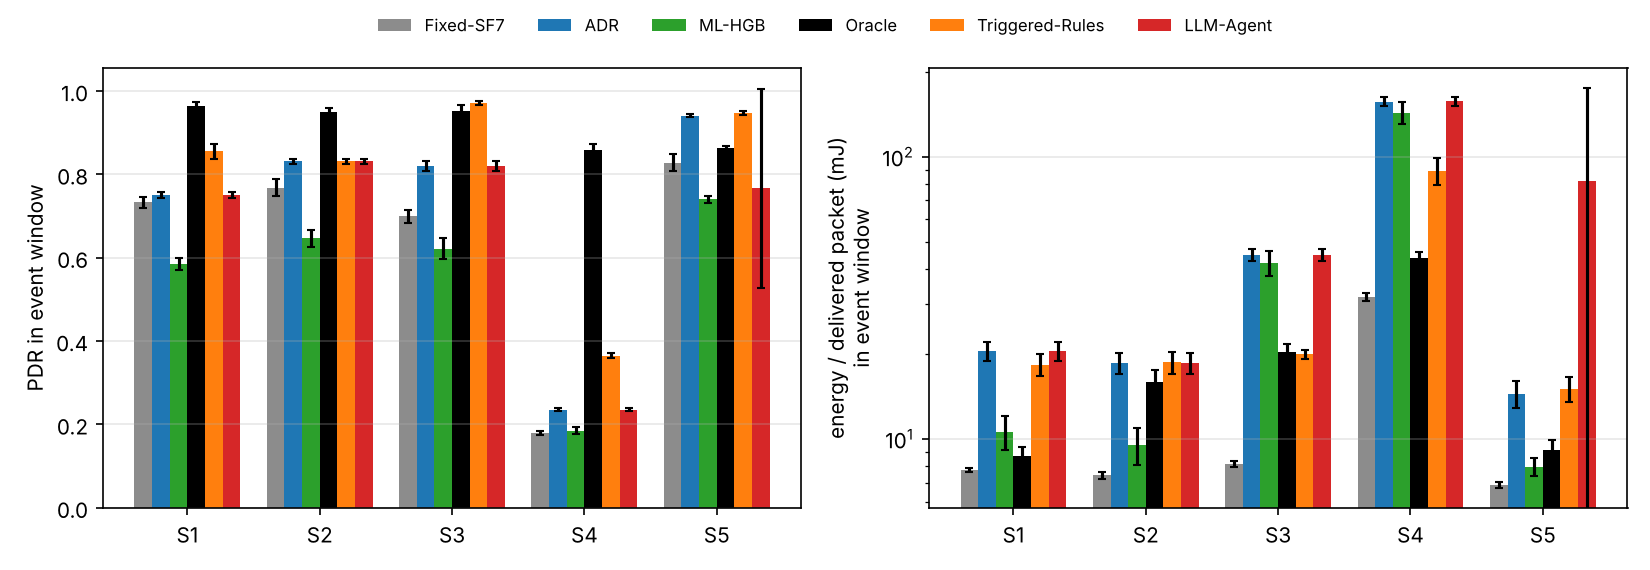
\includegraphics[width=\columnwidth]{../results/e4_event_bars.png}
\caption{E4. Event-window PDR and energy per delivered packet (mean $\pm$ std, 5 seeds).}
\label{fig:e4bars}
\end{figure}
Fig.~\ref{fig:e4} shows the PDR over time and Table~\ref{tab:e4} the event-window PDR with the
paired difference to ADR (same seeds, same channel realisations).

\emph{ADR} keeps the network healthy in normal conditions but does not react to events within
their duration: during jamming its PDR falls to \SOnePdrADR\,\% in the event window and only
recovers when the jammer stops (\SOneRecADR\,min), because ADR can only raise power, never the SF, and
decides on 20-uplink histories.

\emph{Triggered-Rules} --- the same triggers, information and lease mechanism as the agent, with
hand-written rules --- improves the event-window PDR by \SOneDiffRules{} points under jamming,
\SThreeDiffRules{} at the end of the pass and \SFourDiffRules{} during the gateway outage, on every
seed, and halves the energy per delivered packet in S3 (\SThreeERules{} vs \SThreeEADR\,mJ). The
event-triggered architecture is therefore worth about ten points by itself; this is the bar an LLM
agent has to clear. No network-side controller helps against the deep fade (S2,
\STwoDiffRules{} points): under class~A a command needs a delivered uplink, and faded devices are
silent. Only the oracle, which acts instantly and sees the fade, recovers (\STwoDiffOracle{} points).

The \emph{oracle} is the upper bound in S1--S4 but ends \SFiveDiffOracle{} points relative to ADR in
the traffic surge: it minimises the energy of each packet in isolation, which puts most devices on SF7
and multiplies same-SF collisions. The \emph{ML classifier} trained on its labels inherits this
myopia and adds under-provisioning (\SOneDiffML{} points in S1).

\emph{The LLM agent} (Qwen3-0.6B~\cite{qwen3}, \AgentRuns{} runs, \AgentDecisions{} decisions) read the network
correctly with the tools but applied a change only \AgentAppliedTotal{} times; over E3 and E4,
\AgentAppliedTemplate{} of its \AgentAppliedAll{} applied changes were the same action, every device
to SF12 at 10\,dBm. It is identical to
ADR in S1--S3 (\SOneDiffAgent, \STwoDiffAgent{} and \SThreeDiffAgent{} points). In S5 its
event-window PDR was \SFiveDiffAgent{} $\pm$ \SFiveDiffSdAgent{} points relative to ADR, with a loss on
\SFiveLossesAgent{} of 5 seeds: at the
onset of the surge it moved every device to SF12 at 10\,dBm for 30\,min; an SF12 packet occupies
the channel 23 times longer than an SF7 packet, the SF of most devices, while the traffic was five
times higher. In one of the two runs its final message even stated that no change was required. The
action was valid (in range, read-before-write respected), so the
schema guardrail accepted it.



\begin{table}[t]
\caption{E4: event-window PDR (\%, mean $\pm$ std over 5 seeds) and paired difference to ADR (points;
seeds better / worse).}
\label{tab:e4}
\centering\scriptsize
\setlength{\tabcolsep}{2.5pt}
\begin{tabular}{@{}lccccc@{}}
\toprule
& S1 jam & S2 fade & S3 pass end & S4 outage & S5 surge\\
\midrule
ADR & \SOnePdrADR$\pm$\SOnePdrSdADR & \STwoPdrADR$\pm$\STwoPdrSdADR & \SThreePdrADR$\pm$\SThreePdrSdADR & \SFourPdrADR$\pm$\SFourPdrSdADR & \SFivePdrADR$\pm$\SFivePdrSdADR\\
Fixed SF7 & \SOnePdrSFseven & \STwoPdrSFseven & \SThreePdrSFseven & \SFourPdrSFseven & \SFivePdrSFseven\\
Fixed SF12 & \SOnePdrSFtwelve & \STwoPdrSFtwelve & \SThreePdrSFtwelve & \SFourPdrSFtwelve & \SFivePdrSFtwelve\\
ML-HGB & \SOnePdrML & \STwoPdrML & \SThreePdrML & \SFourPdrML & \SFivePdrML\\
Trig.-Rules & \SOnePdrRules & \STwoPdrRules & \SThreePdrRules & \SFourPdrRules & \SFivePdrRules\\
\quad $\Delta$ & \SOneDiffRules{} (\SOneWinsRules/\SOneLossesRules) & \STwoDiffRules{} (\STwoWinsRules/\STwoLossesRules) & \SThreeDiffRules{} (\SThreeWinsRules/\SThreeLossesRules) & \SFourDiffRules{} (\SFourWinsRules/\SFourLossesRules) & \SFiveDiffRules{} (\SFiveWinsRules/\SFiveLossesRules)\\
LLM agent & \SOnePdrAgent & \STwoPdrAgent & \SThreePdrAgent & \SFourPdrAgent & \SFivePdrAgent$\pm$\SFivePdrSdAgent\\
\quad $\Delta$ & \SOneDiffAgent{} (\SOneWinsAgent/\SOneLossesAgent) & \STwoDiffAgent{} (\STwoWinsAgent/\STwoLossesAgent) & \SThreeDiffAgent{} (\SThreeWinsAgent/\SThreeLossesAgent) & \SFourDiffAgent{} (\SFourWinsAgent/\SFourLossesAgent) & \SFiveDiffAgent{} (\SFiveWinsAgent/\SFiveLossesAgent)\\
Oracle & \SOnePdrOracle & \STwoPdrOracle & \SThreePdrOracle & \SFourPdrOracle & \SFivePdrOracle\\
\bottomrule
\end{tabular}
\end{table}

The detector, scored on the ADR runs, reaches an alert precision of \DetPrecision{} and a recall of
\DetRecall{}; it flags jamming within \SOneDetDelay\,min and the outage within \SFourDetDelay\,min, but
the deep fade only after \STwoDetDelay\,min, because faded devices fall silent instead of reporting a
lower SNR.

\subsection{E5 -- Cost of the agent}
\begin{figure}[t]
\centering
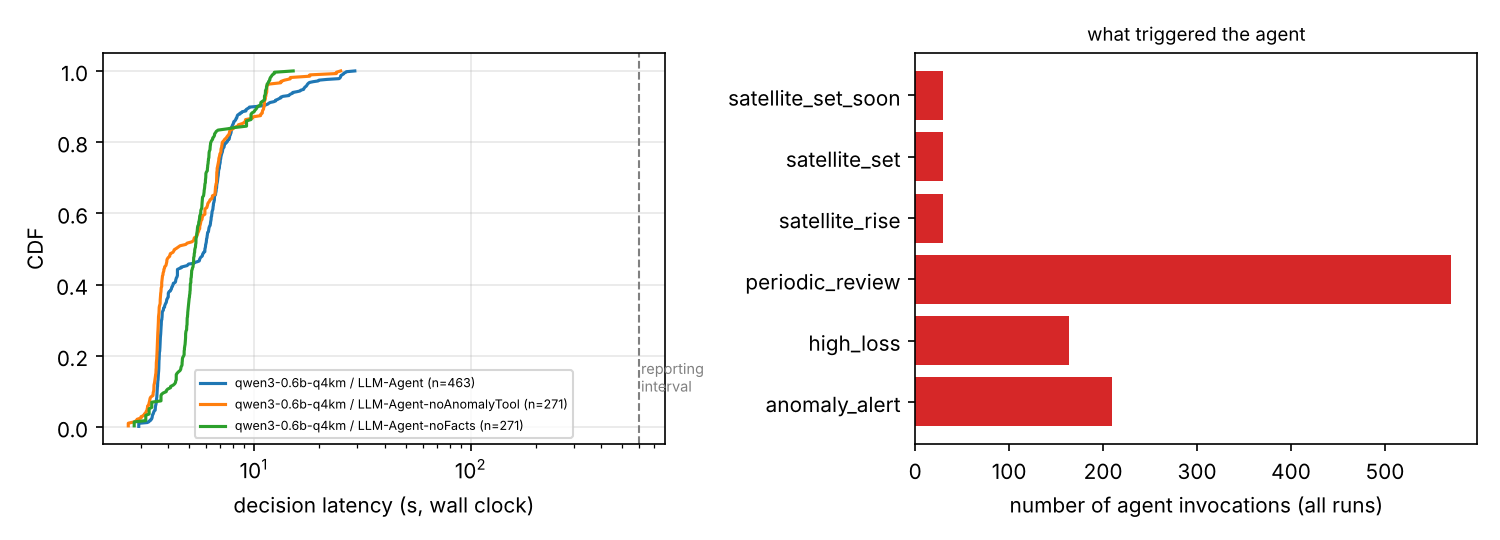
\includegraphics[width=\columnwidth]{../results/e5_agent_cost.png}
\caption{E5. Agent decision latency (CDF, wall clock, 2 CPU threads) and what triggered the agent.}
\label{fig:e5}
\end{figure}
On 2 CPU threads, a decision takes \AgentLatMed\,s (median) and \AgentLatPninetyfive\,s (95th
percentile), with \AgentToolsPerDec{} tool calls and \AgentCallsHour{} LLM calls per simulated hour,
most of them periodic reviews (Fig.~\ref{fig:e5}). This is two orders of magnitude below the 10-min
reporting interval: the reaction delay is set by class-A delivery (up to one reporting period), not
by the model. \AgentSetRejected{} of the \AgentSetCalls{} \texttt{set\_tx\_params} calls were
rejected (invalid-action rate \AgentInvalid\,\%), all for an empty target group; there was no
read-before-write violation (\AgentRbw) and no backend failure.

\subsection{E6 -- Ablations}
Removing the anomaly tool or the LoRa facts from the prompt made the 0.6B model entirely passive:
over \DecisionsNoTool{} and \DecisionsNoFacts{} decisions it applied \AppliedNoTool{} and
\AppliedNoFacts{} changes, read one tool per decision and stopped. Both variants are therefore
identical to ADR in every scenario, including S5 (\SFivePdrNoTool\,\% and \SFivePdrNoFacts\,\% against
\SFivePdrAgent\,\% for the full agent, Fig.~\ref{fig:e6}). For this model, the context that makes it
act is also what makes it harmful; an ablation can only show the value of a component if the full
agent has some, which a larger model may provide.

\begin{figure}[t]
\centering
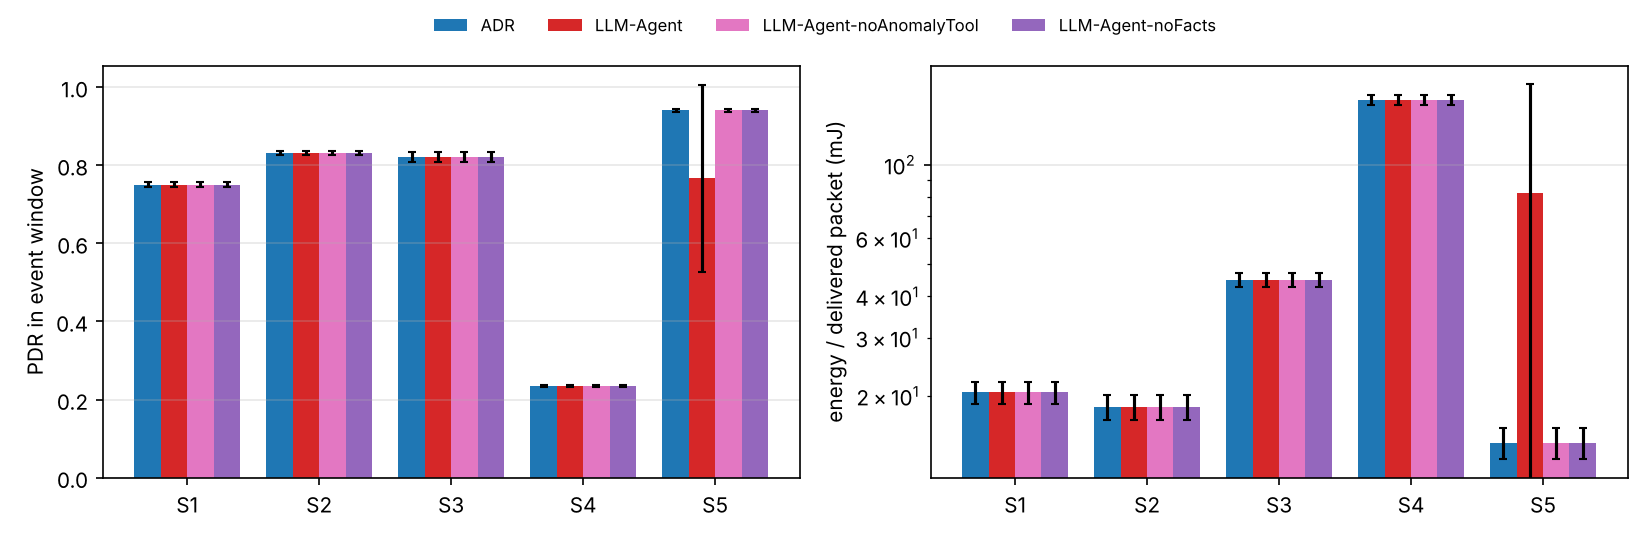
\includegraphics[width=\columnwidth]{../results/e6_ablations.png}
\caption{E6. Event-window PDR and energy per delivered packet for ADR, the full agent and the two
ablations (Qwen3-0.6B, 5 seeds).}
\label{fig:e6}
\end{figure}

